\newpage
\section{Edge Detection in Images} 
Edges in images are discontinuities in intensity. They usually represent the boundaries of objects or lighting present in the image.
It is one of the first steps in object detection models.

Edges can be typically classified into Step, Ramp and Roof edges. A step edge represents an abrupt change in intensity, where the image intensity transitions from one value to another in a single step. A ramp edge describes a gradual transition in intensity over a certain distance rather than an abrupt change. A roof edge represents a peak or ridge in the intensity profile, where the intensity increases to a maximum and then decreases.

\begin{figure}[H]
    \centering
    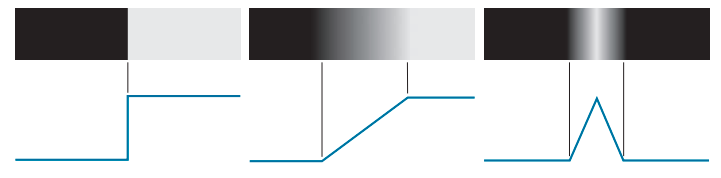
\includegraphics[width=0.5\linewidth]{Figures/1/edges.png}
    \caption{Types of edges found in an image. \textit{Source: Digital Image Processing by R. C. Gonzalez \& R. E. Woods}}
\end{figure}

Here, we will attempt to build an algorithm that can detect any of these edges using the principles of numerical differentiation.

\subsection{Algorithm and Theoretical Approach}
The most straightforward algorithm for finding the edges in any image involves the following processes.

\begin{enumerate}
    \item Conversion of an RGB image into a grayscale image. This is to flatten the 3-dimensional array into a 2-dimensional one to make it easier to work with. The standard formula for the conversion is
    \begin{align}
        \text{Gray} = 0.3\cdot\text{Red} + 0.59\cdot\text{Green} + 0.11\cdot\text{Blue}
    \end{align}
    This formula closely represents the average person's relative perception of the brightness of red, green, and blue light.
    \item Consider the greyscale image as a plot of a multivariable function $G(x, y)$ where the ordered pair $(x, y)$ is the pixel location and the output $G(x, y)$ is the value of the grey scale at that point. Finding the gradient at each pixel in the grid grid represents the change in intensity at every pixel.
    \item Fixing a threshold value ($\delta$) and classifying all pixels with values $||\nabla G(x,y)||>\delta$ as an edge.
\end{enumerate}

\subsubsection{Gradient of a 2D Scalar Field}
The gradient of a 2D scalar matrix will give us the overall change in intensity around every point. If $G$ represents our scalar matrix, the gradient at any point $(i,j)$ can be written as,

\begin{align} \label{1grad}
\nabla G \approx \biggl \langle \frac{G(x+1,y)-G(x-1,y)}{2} , \frac{G(x,y+1)-G(x,y-1)}{2}\biggl \rangle 
\end{align}

where we used the central difference scheme for the first derivative with $h=1$. 

\begin{align} \label{firstderivative}
    f'(x) = \frac{f(x+h)-f(x-h)}{2h}
\end{align}

However, pixels could be tightly packed in an image, and a point's immediate neighbours may not have enough contrast to truly detect edges. Furthermore, in Eq. \ref{1grad}, notice that we only use 4
of the 8 neighbors of the pixel $(i,j)$. The algorithm could be even more precise if we could somehow include information about pixels further away than 1 pixel.

Using the Taylor series expansion,

\begin{align}
    f(x+h) = f(x) + f'(x)h + \frac1{2}f''(x)h^2 +\frac1{6}f'''(\xi_3)h^3,\\f(x-h) = f(x) - f'(x)h + \frac1{2}f''(x)h^2 -\frac1{6}f'''(\xi'_3)h^3\\
    \implies \frac{f(x+h)-f(x-h)}{2h} = f'(x) + \frac{1}{3}f'''(x)h^2 + ...
\end{align}

By putting changing $h \rightarrow 2h$ and adding both the summations, we get (for $h=2$)

\begin{align} \label{edge2}
    f'(x) = \frac{8\left[f(x+1)-f(x-1)\right] - \left[f(x+2)-f(x-2)\right]}{12}
\end{align}

% Adding this to the value for $h=1$, we get

% \begin{align} \label{edge21}
%     2f'(x) = \frac{f(x+2)-f(x-2)}{4} + \frac{f(x+1)-f(x-1)}{2}\\
%     \text{or, }f'(x) = \frac{2f(x+1)+f(x+2)-2f(x-1)-f(x-1)}{8}
% \end{align}

\noindent All the centred finite difference schemes will have an error of $O(h^2)$ associated with them.

One can apply a simple blur to the image before edge detection to reduce the fine noise by averaging every pixel value with its 8 neighbours.

\subsubsection{Second Derivatives}

% The edge detection methods which used the first derivative can result in the detection of too many edge points since we are classifying anything above a threshold value an edge. 
As we have seen in the previous section, the local maxima/minima in gradient values represent edge points. This means that at edge points, there will be a peak in the first derivative, and equivalently, there will be a zero crossing in the second derivative. Thus, edge points may be detected by finding the zero crossings of the second derivative of the image intensity.

The simplest way to find the second derivate of a scalar matrix is to find its Laplacian. Using the Taylor series expansion mentioned earlier, we can calculate the second derivate of a function as 

\begin{align}
    f''(x) = f(x+h)+f(x-h)-2f(x)
\end{align}

Thus, the two-dimensional Laplacian will be,

\begin{align}
    \nabla^2 G(x,y) = \frac{1}{h^2}\left(G(x,y+1)+G(x,y-1)+G(x-1,y)+G(x-1,y)-4G(x,y)\right)
\end{align}

However, the problem with this approach is that even very small local peaks in the first derivative will result in zero crossings in the second derivative, making them extremely sensitive to noise.

The zero crossings can be found by multiplying a pixel value with its neighbour and checking if the product is $<0$.
% Therefore, it is desirable to filter out the noise before edge enhancement. To do this, the Laplacian of Gaussian (LoG) combines Gaussian filtering with the Laplacian for edge detection.

% Convolve with gaussian filter then perform laplacian test

\subsection{Implementation}

\begin{lstlisting}[language=Python, caption=Code implementing edge detection techniques and related functions as discussed above]
import numpy as np
import matplotlib.pyplot as plt

# RGB to grayscale conversion
def rgb2gray(rgb):
    return np.dot(rgb[...,:3], [0.3, 0.59, 0.11])

# Image blur
def blur(img):
    n = img.shape
    smooth = img.copy()
    # we ignore the edges as they are just 1 pixel
    for x in range(1, n[0]-1):
        for y in range(n[1]-1):
            smooth[x,y] = (img[x,y]+img[x-1,y]+img[x+1,y]+\
                           img[x,y-1]+img[x-1,y-1]+img[x+1,y-1]+\
                           img[x,y+1]+img[x-1,y+1]+img[x+1,y+1])/9
    return smooth

# A simple masking function for display
def mask(img, k=0.25):
    mk = np.where(img > k*np.max(img), 1, 0)
    return mk

# Gradient of G using the Nabla operator
def nablaG(G,x,y,h=1):
    if h == 1:
        delx = (G[x+1,y]-G[x-1,y])/2
        dely = (G[x,y+1]-G[x,y-1])/2
    elif h == 2:
        delx = (8*G[x+1,y]-G[x+2,y]-8*G[x-1,y]+G[x-2,y])/12
        dely = (8*G[x,y+1]-G[x,y+2]-8*G[x,y-1]+G[x,y-2])/12
    else: 
        return (0, 0)
    return (delx, dely)

def gradient(img, h=1, file=False):
    grad = np.zeros((img.shape[0], img.shape[1]), dtype=float)
    for x in range(h, img.shape[0]-h):
        for y in range(h, img.shape[1]-h):
            g = nablaG(img, x, y, h=h)
            grad[x, y] = np.sqrt(g[0]**2+g[1]**2)
    return grad

# Calculate the Laplacian of a matrix
def laplacian(img, h=1):
    lap = np.zeros((img.shape[0], img.shape[1]), dtype=float)
    for x in range(h, img.shape[0]-h):
        for y in range(h, img.shape[1]-h):
            lap[x, y] = (img[x,y+1]+img[x,y-1]+img[x+1,y]+img[x-1,y]-4*img[x,y])/h**2
    return lap

# Find the zero crossings           
def zero_crossings(img):
    mk = np.ones((img.shape[0],img.shape[1]))
    # zero crossings are given a value 0, the others 1.
    for x in range(1, img.shape[0]-1):
        for y in range(1, img.shape[1]-1):
            pix = img[x,y]
            if pix*img[x-1,y] < 0 or pix*img[x+1,y] < 0 or pix*img[x,y+1] < 0 or pix*img[x,y-1] < 0:
                mk[x,y] = 0
    return mk

# performing edge detection on a sample
img_rgb = mpimg.imread(f'data/pic.png')
img = rgb2gray(img_rgb)
grad = blur(gradient(img, h=2))
plt.figure()
plt.imshow(mask(grad, k=0.3), cmap = 'gray')
plt.show()
\end{lstlisting}

\subsection{Results}
After calculating the corresponding gradient matrix, 
Figures \ref{edge1} to \ref{edge3} show edge detection performed on three different images using the first derivative approach (i.e. using the gradient matrix) compared with the industry standard \textit{Canny} Edge Detection algorithm using \verb|OpenCV|.

\begin{figure}[H]
    \centering
    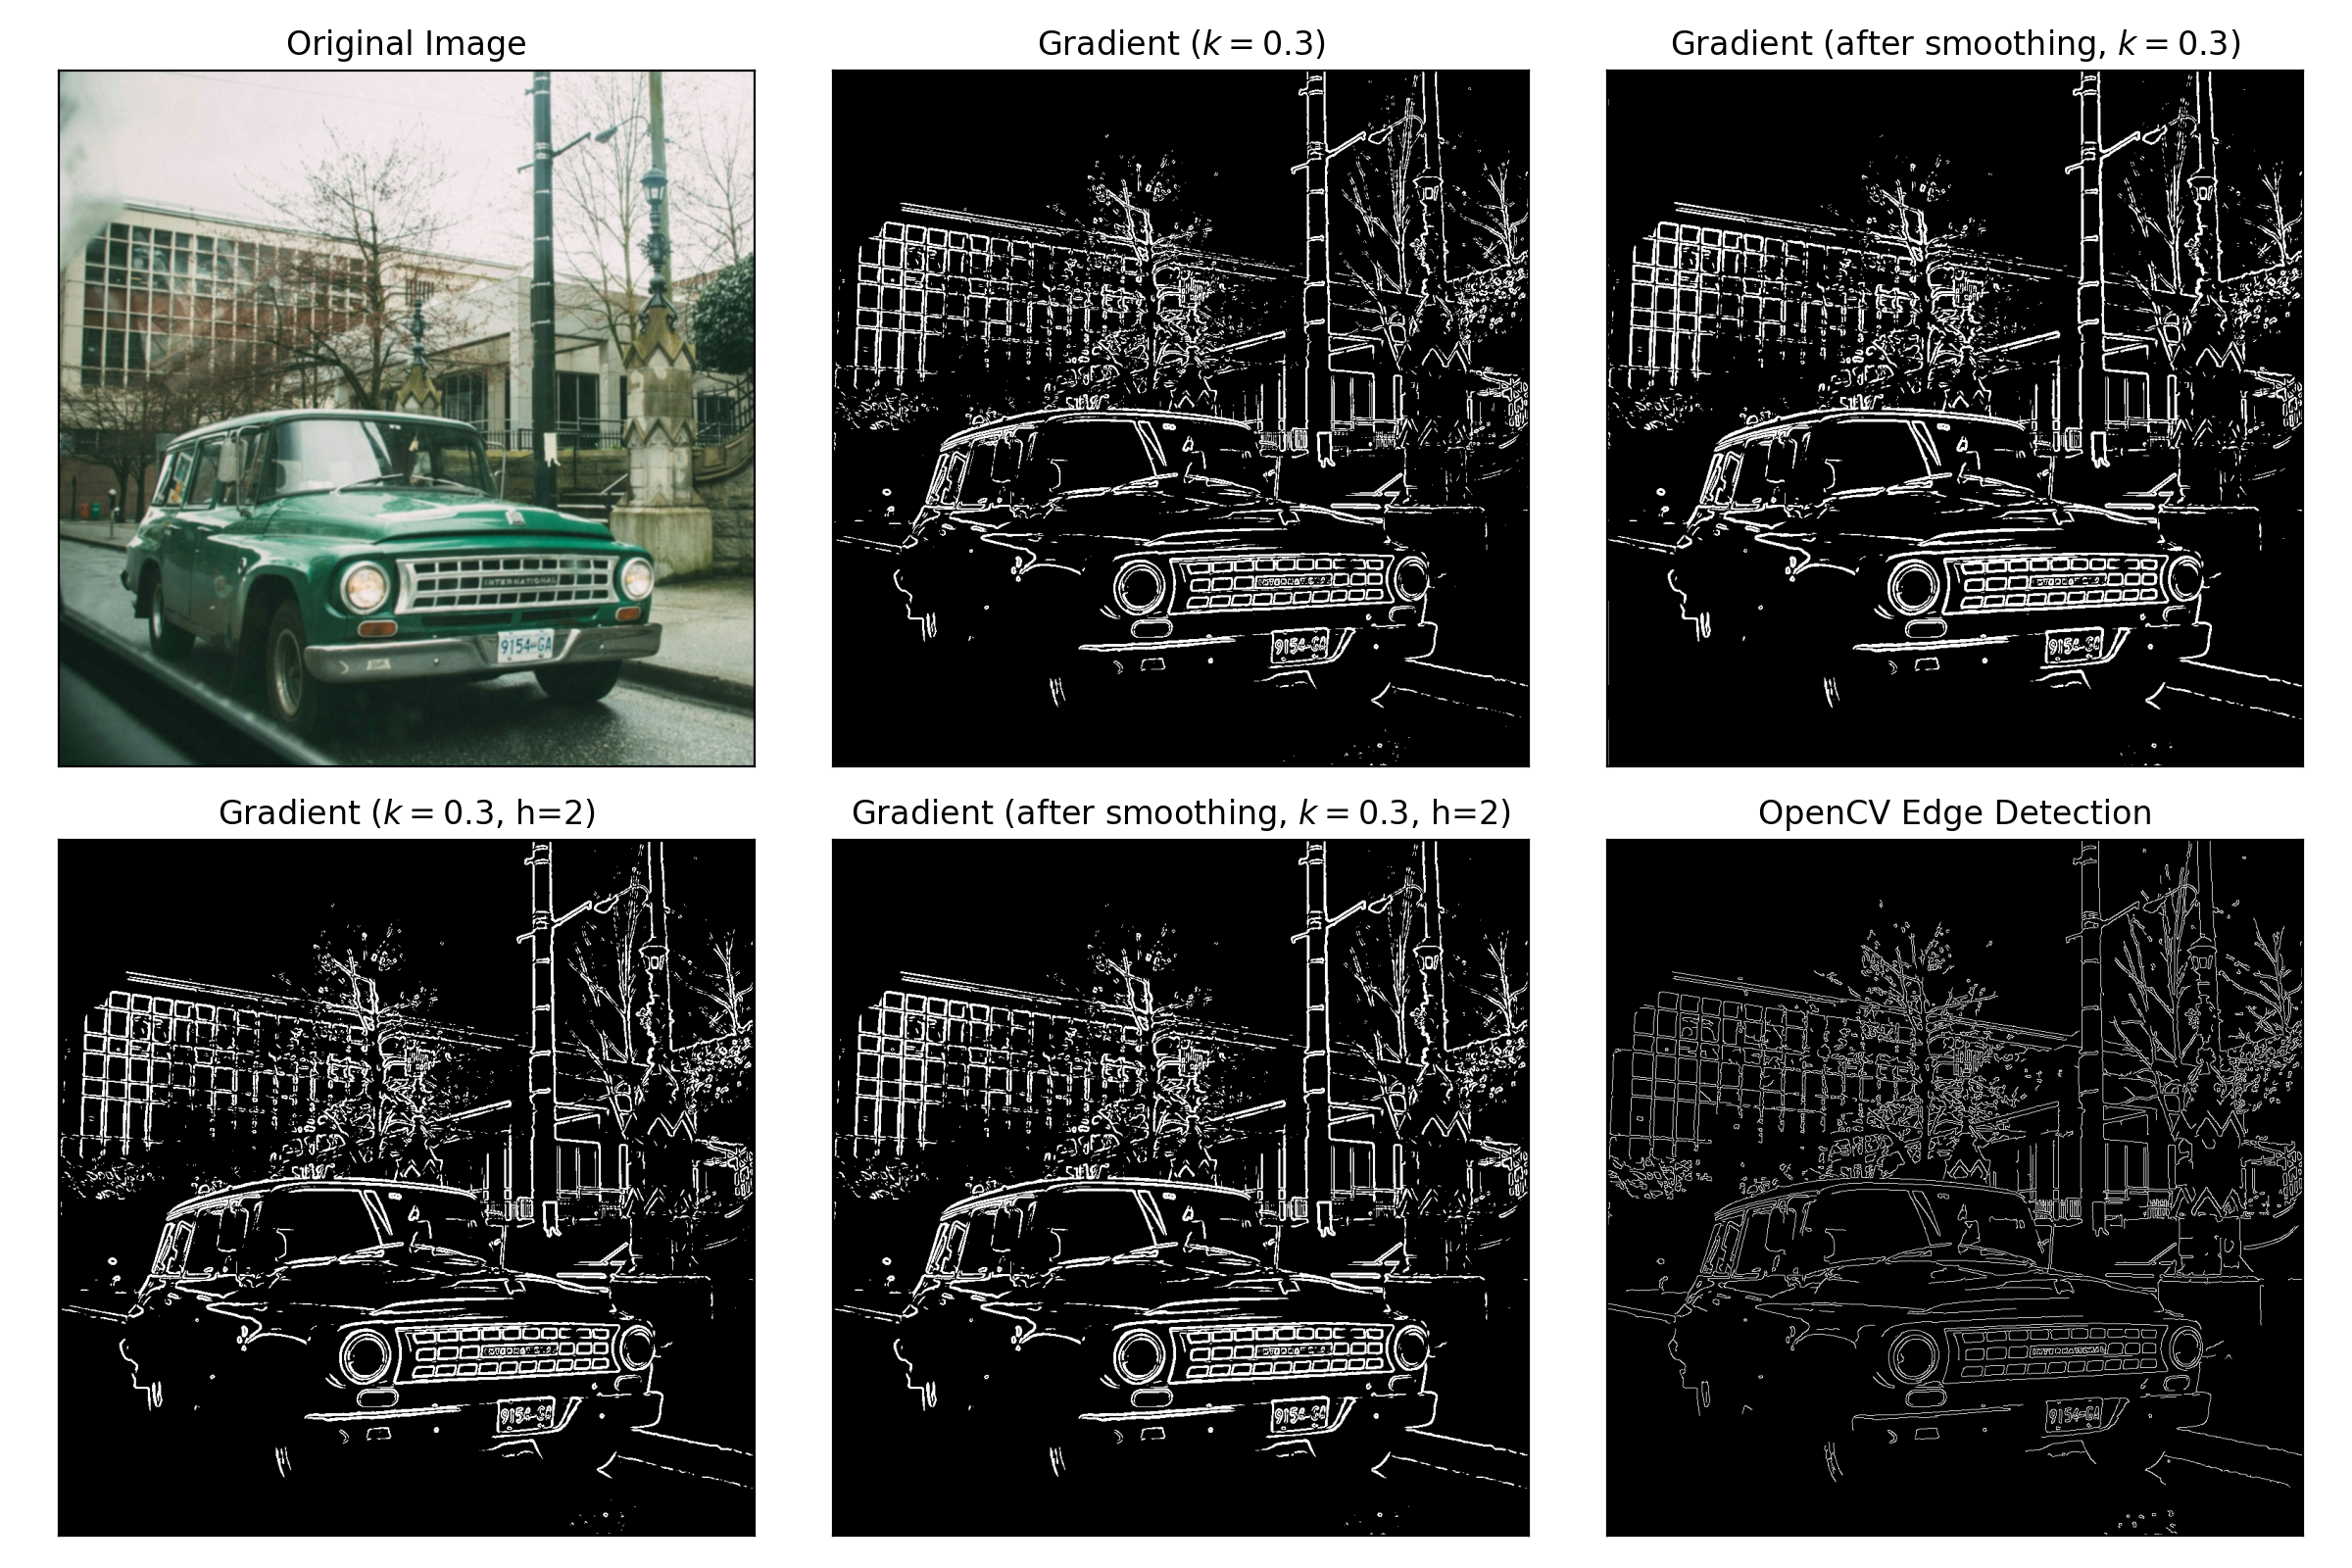
\includegraphics[width=1\linewidth]{Figures/1/cara.png}
    \caption{Edge detection results by altering various parameters as mentioned for an image}
    \label{edge1}
\end{figure}

\begin{figure}[H]
    \centering
    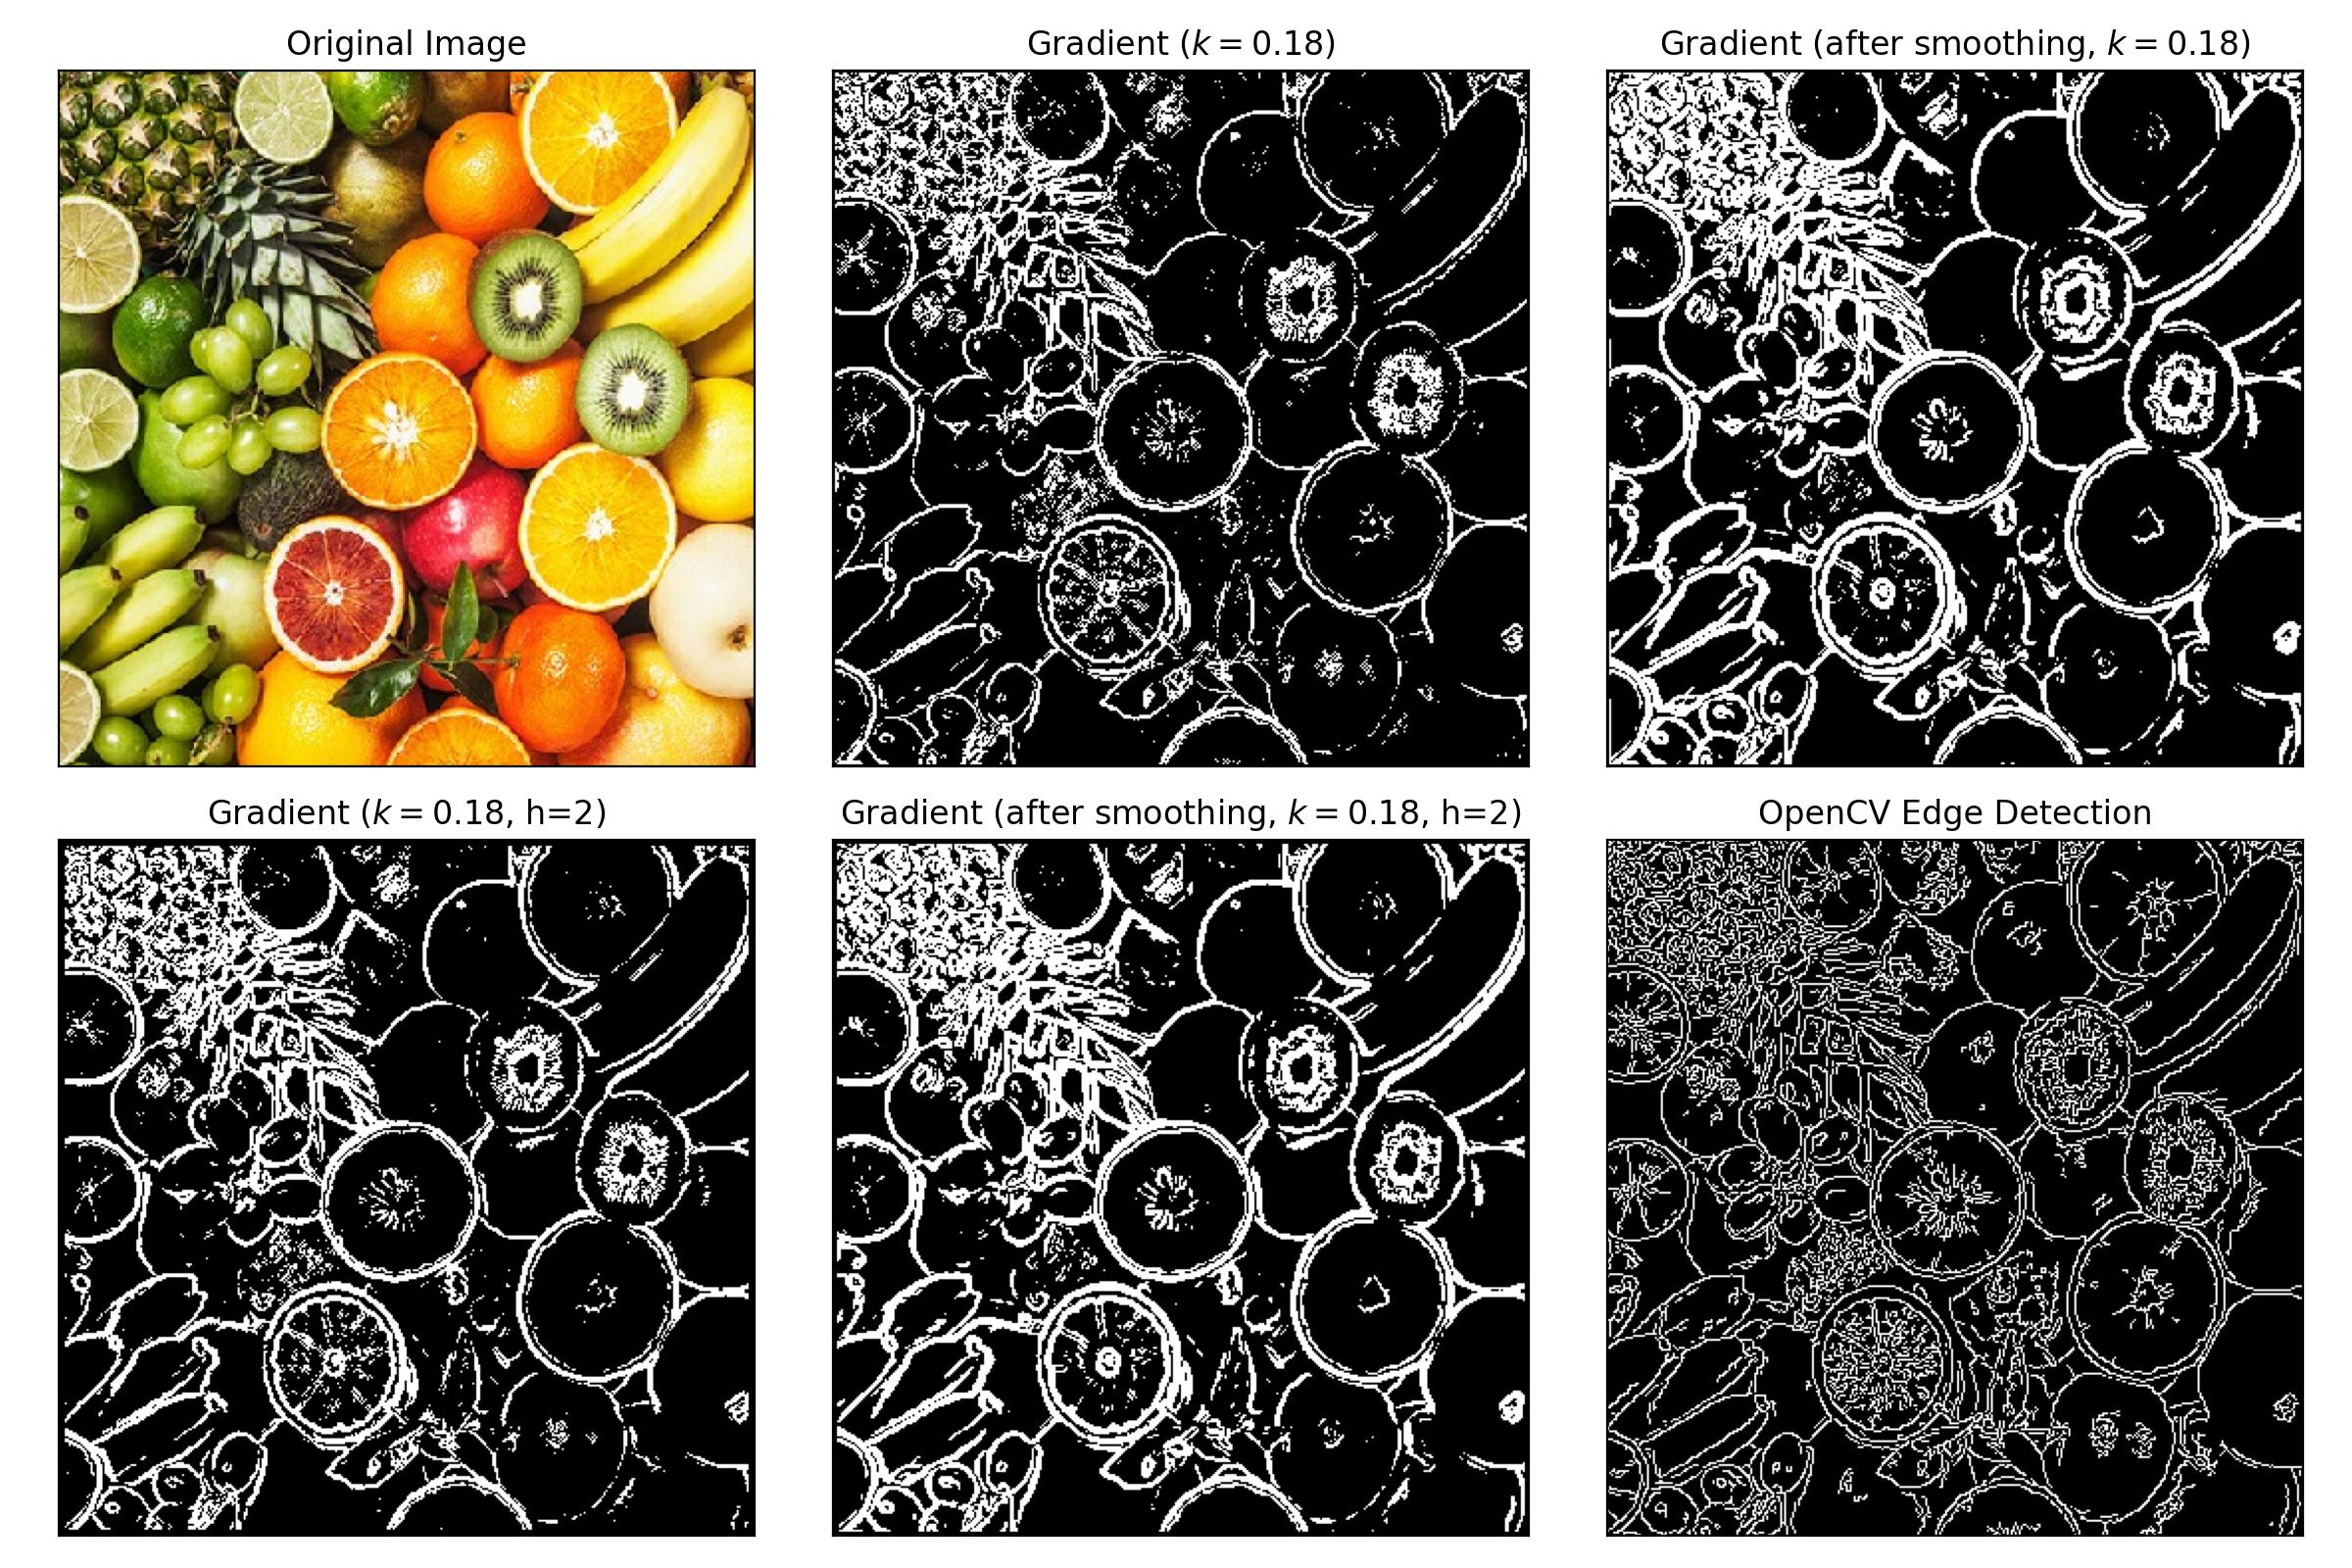
\includegraphics[width=1\linewidth]{Figures/1/fruits.jpg}
    \caption{Edge detection results by altering various parameters as mentioned for an image}
\end{figure}

\begin{figure}[H]
    \centering
    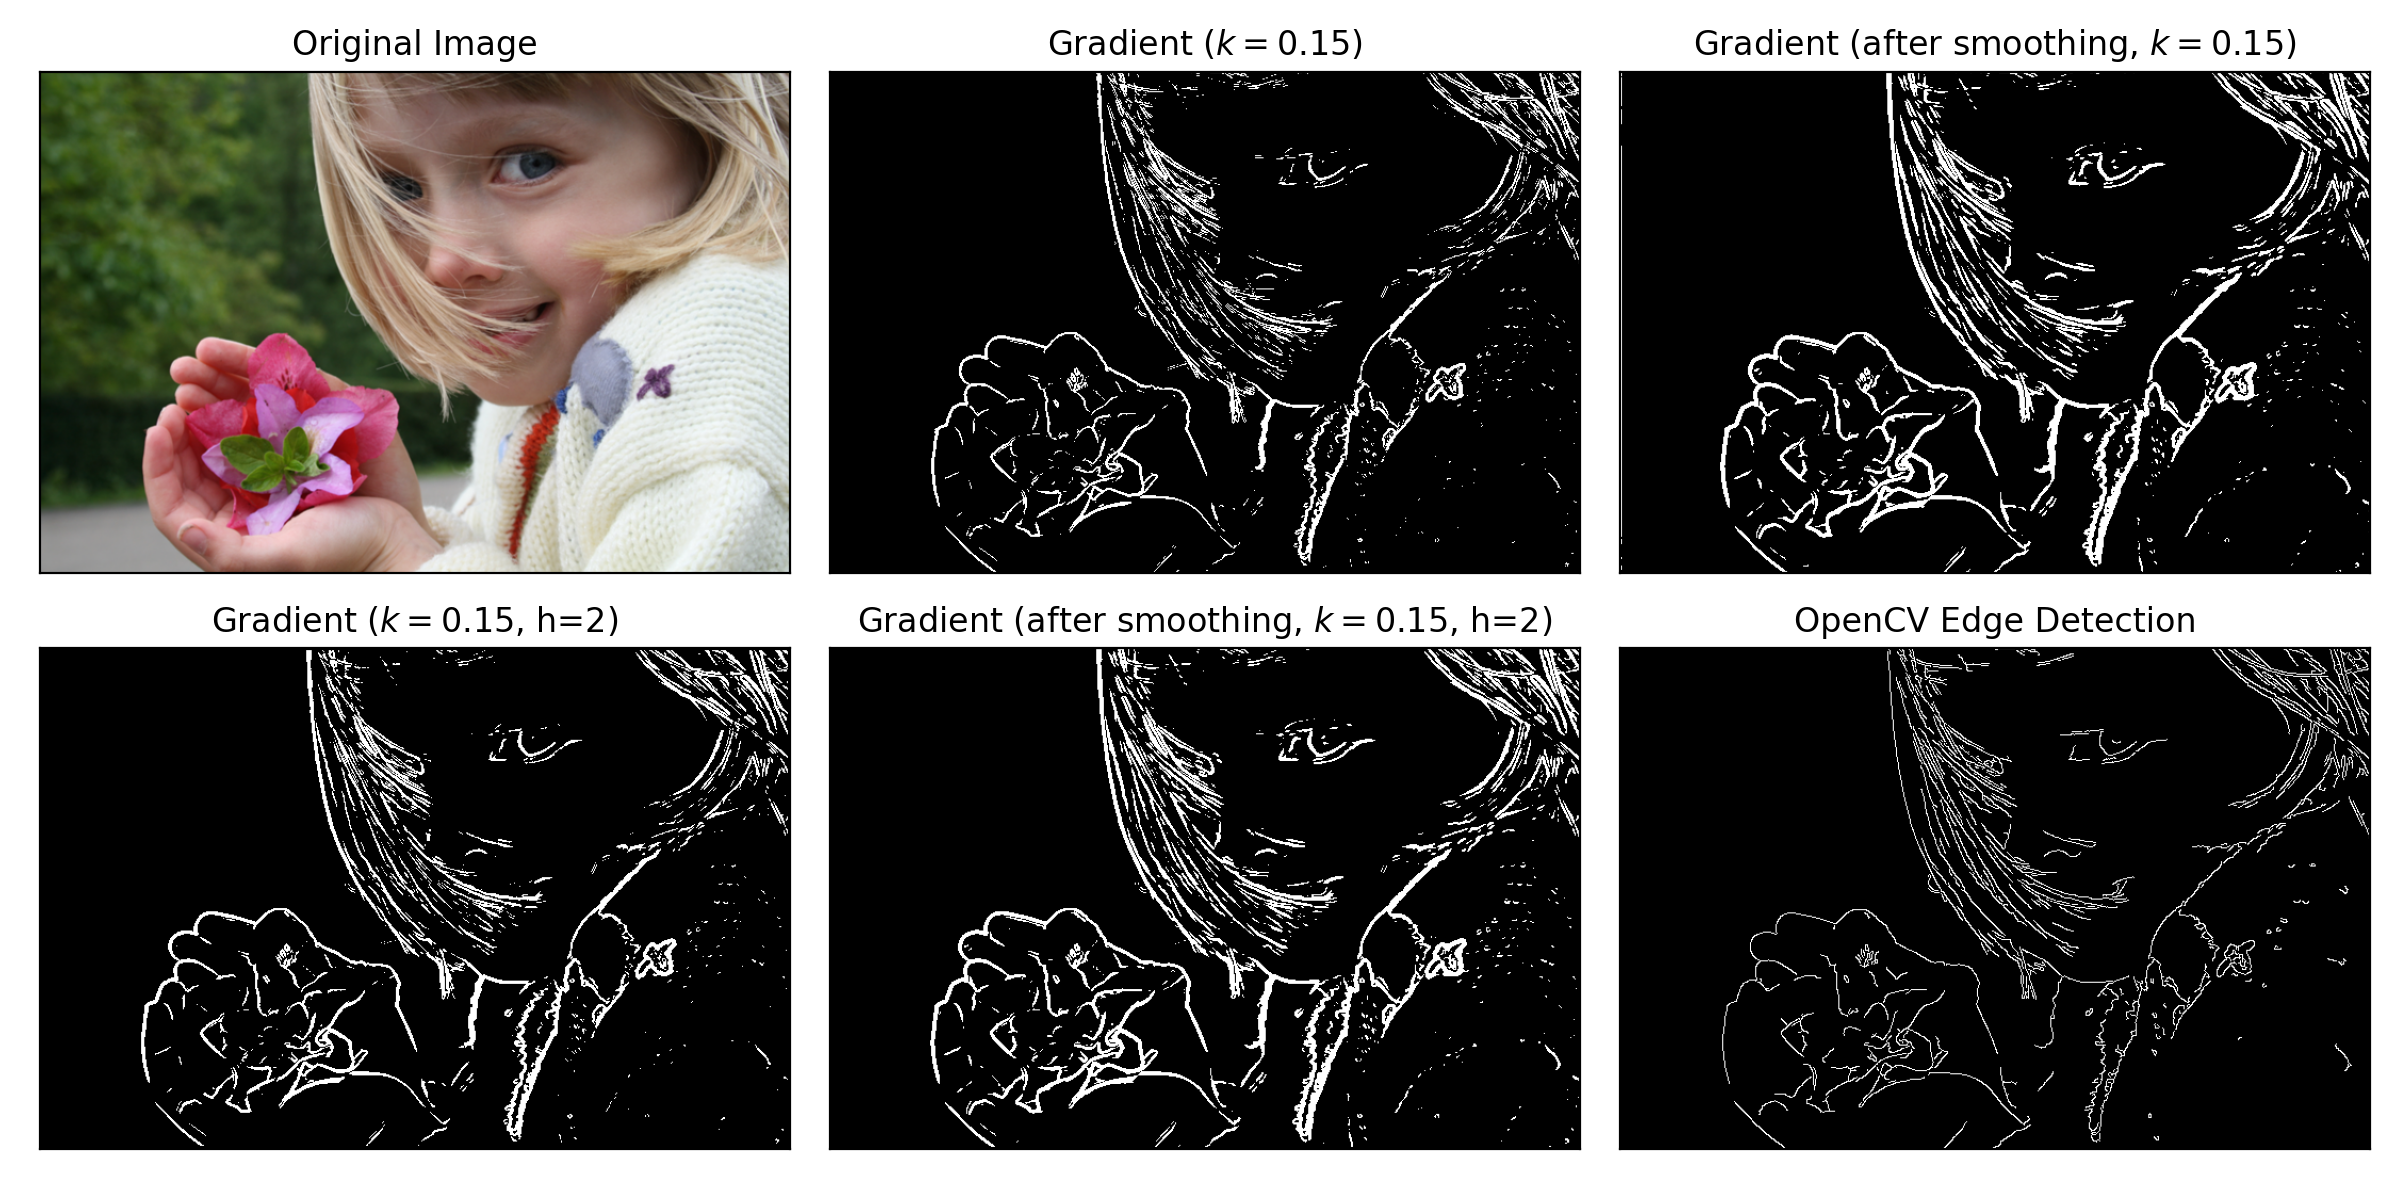
\includegraphics[width=0.8\linewidth]{Figures/1/kid.png}
    \caption{Edge detection results by altering various parameters as mentioned for an image}
    \label{edge3}
\end{figure}

Figure \ref{edge4} shows edge detection performed using the second derivative approach, i.e. finding the zero crossings of the Laplacian. These images were first passed through the \verb|blur()| function.

\begin{figure}[H]
    \centering
    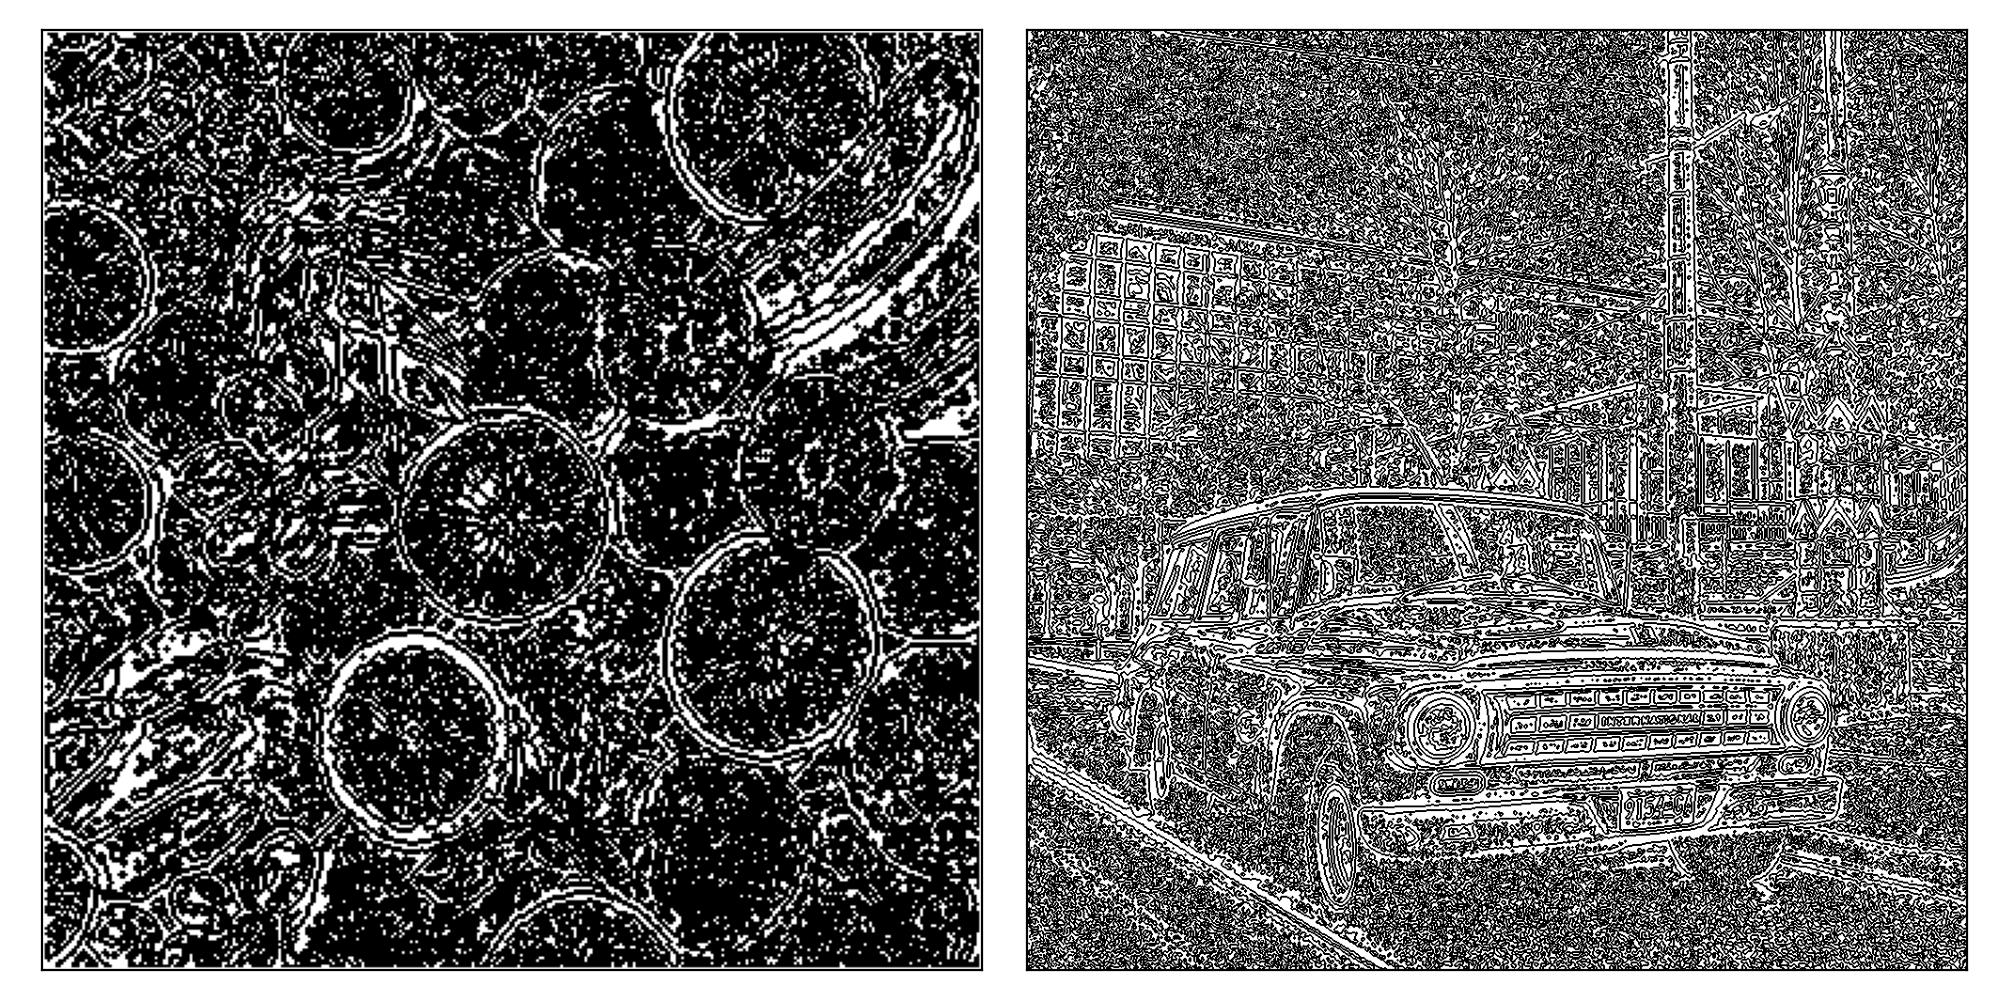
\includegraphics[width=0.7\linewidth]{Figures/1/edge2.jpg}
    \caption{Zero crossings of the Laplacian for two of the images used above.}
    \label{edge4}
\end{figure}

As you can see, these results are not as good as the ones we obtained with the first approach. This is due to the high amount of noise in the image creating a lot of local extremum points (even after smoothing), which get detected by the zero crossing algorithm. 

\subsection{Discussion}
%small operator good localisation but sensitive to noise

In this project, we have explored different kinds of edge detection algorithms that use the principle of numerical differentiation. We have seen that the gradient approach (using first derivatives) works much better than the laplacian approach (using second derivatives) due to the high amount of local extremum points caused by noise. However, Laplacian is a very useful tool in blob detection and feature transformation algorithms, which are beyond the scope of this project.

We have also explored including more than the immediate neighbouring pixels in the calculation of derivatives. From the results, we can see that while this marginally reduces the noise in the edges detected, it also reduces the accuracy of the edges. A similar thing is seen when a blur filter is applied before the edge detection -- the thickness of the edges increases.

The standard edge detection algorithm, on the other hand, tries to fix these shortcomings by calculating directional gradients separately and also using hysteresis to detect continuous edges.

Additionally, there are many ways to include 4 corner edges into our gradient. The \textit{Sobel} and \textit{Prewitt} operators are popular methods which use convolution filters to find the horizontal and vertical changes in intensity.

%by two kernels as follows. Without getting into details about convolution, the derivative form of the Sobel operator looks like,

%\begin{align}
   % \nabla G|_x \propto 2G(x-1,y)+G(x-1,y-1)+G(x-1,y+1)-2G(x+1,y)-G(x+1,y-1)+G(x+1,y+1)
%\end{align}